%---------------------------------------------------------------------------%
%-> Frontmatter
%---------------------------------------------------------------------------%
%-
%-> 生成封面
%-
\maketitle% 生成中文封面
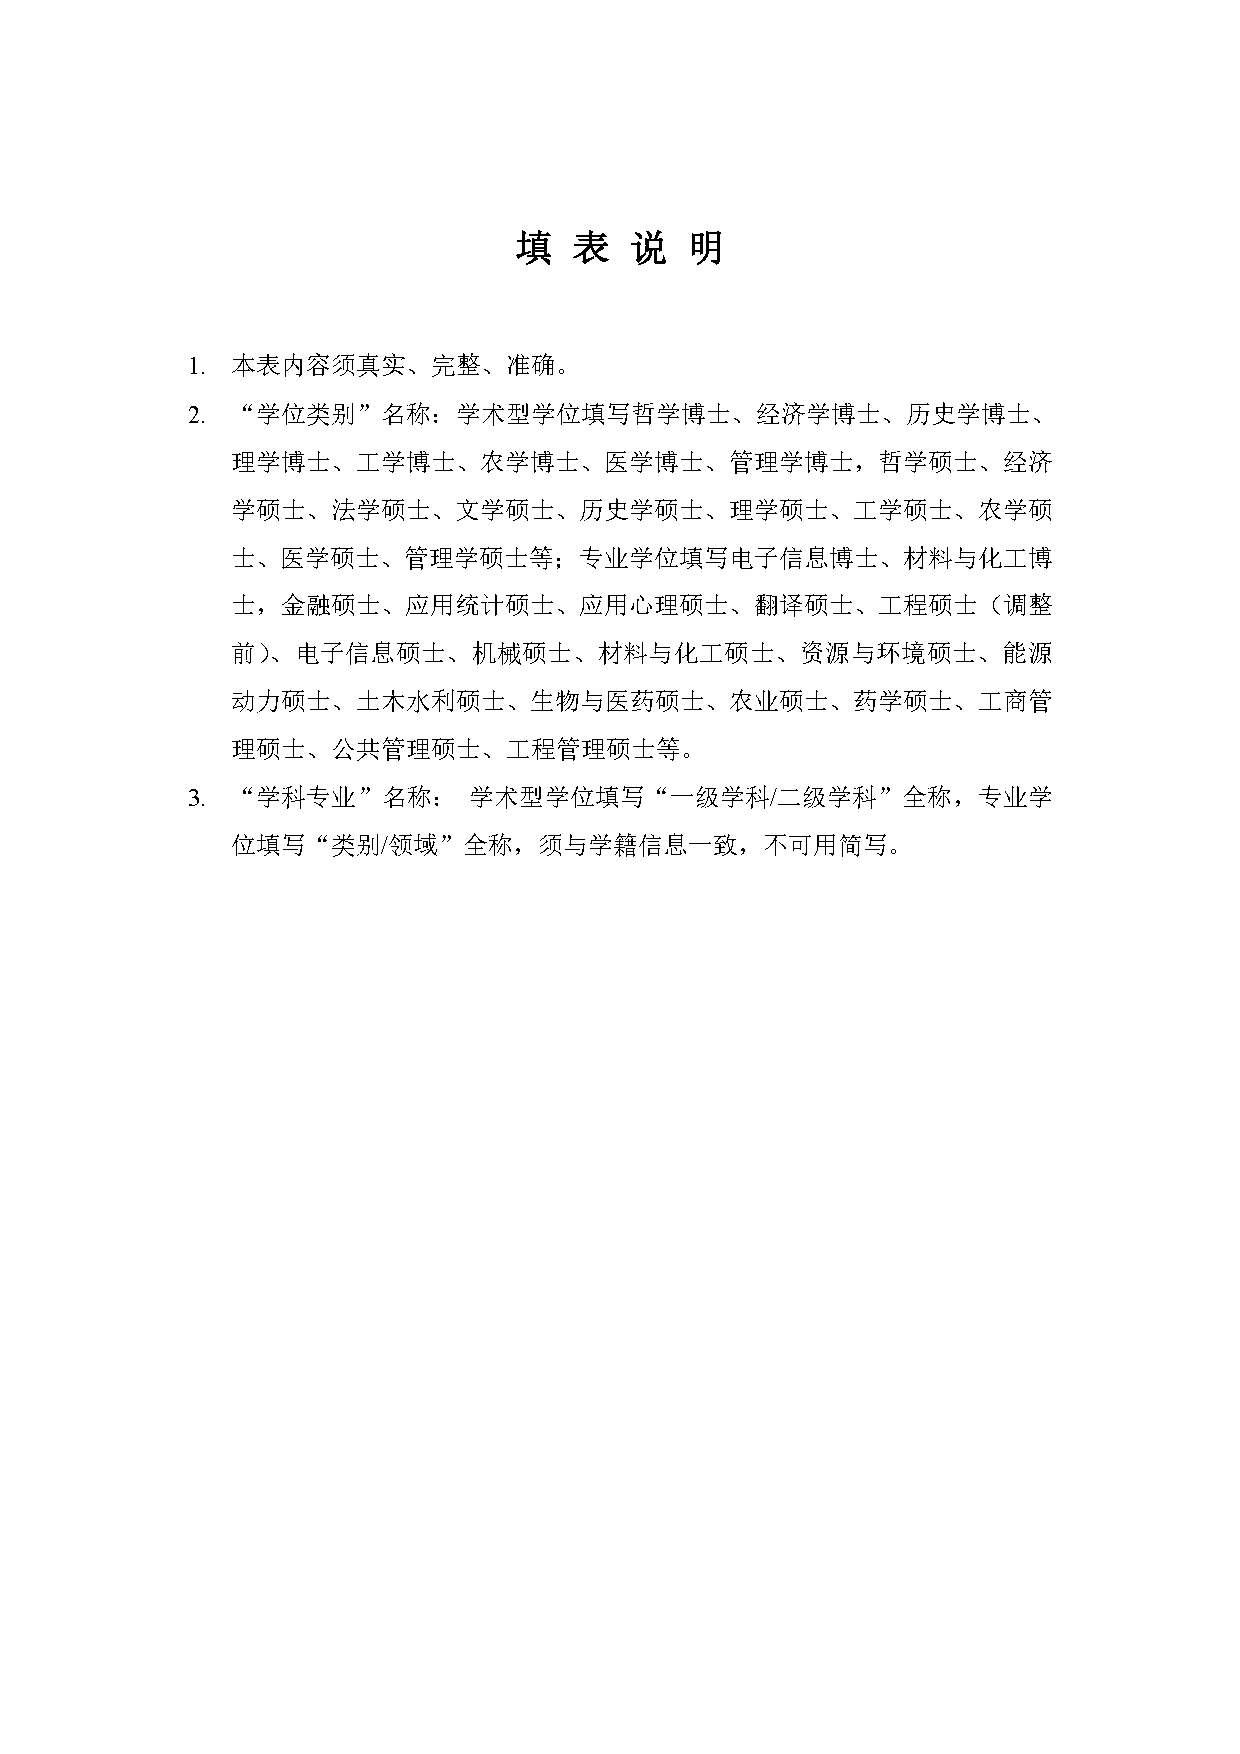
\includepdf[pages={1}, pagecommand={}]{Style/研究生学位论文中期报告-填表说明.pdf}
\newpage
% 空白页

% \newpage
% \thispagestyle{empty}
% \mbox{}


% ----------------摘要-------------------------
\renewcommand{\abstractname}{\bfseries\zihao{4}摘 \quad 要}

\fancypagestyle{abstractpage}{
    \fancyhf{} % 清空页眉页脚
    \fancyhead[C]{\footnotesize 摘要}
}

\begin{abstract}
    \thispagestyle{abstractpage}
    \zihao{-4}  % 设置摘要正文为宋体小4号字
    这里是摘要的正文内容。摘要需要简要说明研究的目的、方法、结果和结论。
\end{abstract}
\noindent \textbf{关键词:} 关键词1, 关键词2, 关键词3
% --------------------------------------------


\newpage
\thispagestyle{empty}
\mbox{}
\newpage

% ----------------英文摘要-------------------------
\renewcommand{\abstractname}{\bfseries\zihao{4} Abstract}

\fancypagestyle{abstractpage}{
    \fancyhf{} % 清空页眉页脚
    \fancyhead[C]{\footnotesize Abstract}
}

\begin{abstract}
    \thispagestyle{abstractpage}
    \zihao{-4}  % 设置摘要正文为宋体小4号字
    Here is the text of the abstract. The abstract needs to briefly describe the purpose, methods, results, and conclusions of the study.
\end{abstract}
\noindent \textbf{Keywords:} University of Chinese Academy of Sciences (UCAS), Thesis,
% --------------------------------------------


\newpage
\thispagestyle{empty}
\mbox{}
\newpage

%-> 目录
\fancypagestyle{tocpage}{
    \fancyhf{} % 清空页眉/页脚
    \fancyhead[C]{\footnotesize 目录}
}

\tableofcontents% 生成目录
\thispagestyle{tocpage}
\newpage

% 空白页

\newpage
\thispagestyle{empty}
\mbox{}


%---------------------------------------------------------------------------%
